\documentclass{beamer}

\usecolortheme[dark,accent=cyan]{solarized}

\beamertemplatenavigationsymbolsempty

\usepackage{coloremoji}
\usepackage{graphicx}
\usepackage{hyperref}
\usepackage{colortbl, xcolor}
\usepackage{booktabs}
\usepackage{varwidth}
\usepackage{hyperref}

\usepackage{tikz}
\usetikzlibrary{positioning,calc}
\usetikzlibrary{automata}
\usepackage{pstricks}
\usepackage{minted}

\definecolor{DarkGray}{gray}{0.1}
\definecolor{DarkGray}{gray}{0.1}
\usemintedstyle{native}

\title{Accessing open research literature with Python}
\author{@NikoletaGlyn}
\date{ }
\institute[]
{
\begin{center}
    \includegraphics[width=.15\textwidth]{static/cardiff_uni_logo.jpg}
\end{center}
}

\begin{document}

\frame{\titlepage}

\begin{frame}
    \begin{center}
    \tikzstyle{arrow} = [thick,->,>=stealth]

\begin{center}
\begin{tikzpicture}

\draw (0, 0) circle (3cm);
\draw[blue!70,fill=blue!70] (0, 0) circle (0.5cm);
\draw[line width=1mm, yellow!70](0, 0) circle (0.8);
\draw [arrow, line width=0.5mm, red!70] (0.5, 0.7) -- (0.7, 1);
\draw [arrow, line width=0.5mm, red!40] (0.5, 0.7) -- (0.7, 1);
\draw [arrow, line width=0.5mm, red!60] (0.7, 1) -- (.95, 1.4);

\draw [arrow, line width=0.5mm, red!80] (0.95, 1.4) -- (1.67, 2.5);

\end{tikzpicture}
\end{center}
\tiny{http://matt.might.net/articles/phd-school-in-pictures/}
    \end{center}
\end{frame}


\begin{frame}
    \begin{center}
    \huge{Scholarly Databases}
    \end{center}
\end{frame}

\begin{frame}
    \begin{center}
    \huge{API}
    \end{center}
\end{frame}

\begin{frame}[fragile]
    \begin{center}
    \textbf{QUERY} \\
    \vspace{3mm}
    \small{\url{http://ieeexplore.ieee.org/gateway/ipsSearch
    .jsp?ti=Namibia&hc=100}} \\
    \pause
    \vspace{10mm}
    \small{\url{http://api.plos.org/search?q=title:Namibia&rows=100}} \\
    \pause
    \vspace{10mm}
    \small{\url{http://www.nature.com/opensearch/request?queryType=cql&query=dc
    .title%20adj%20Namibia&maximumRecords=100}} \\
    \small{...}
    \end{center}
\end{frame}

\begin{frame}
    \begin{center}
    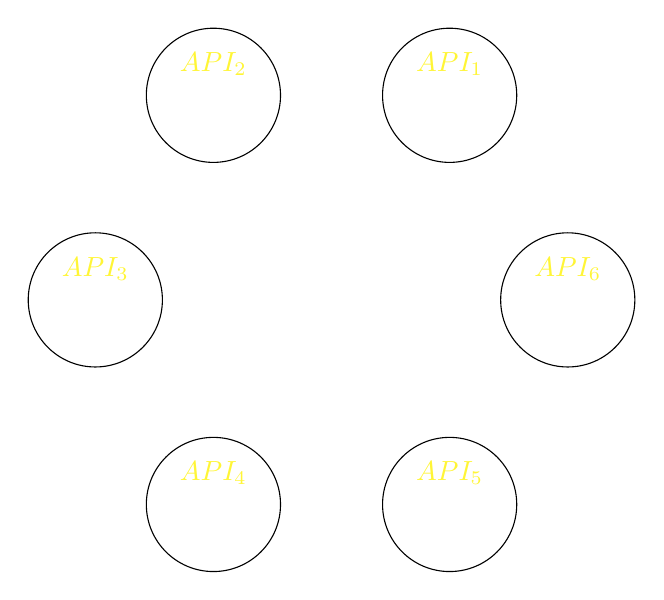
\begin{tikzpicture}

\foreach \phi in {1,...,6}{
    \node[state, align=center] (v_\phi) at (360/6 * \phi:3cm) {\color{yellow!79}$API_\phi$ \\\color{white!79}\tiny{Query}
    \\ \color{white!79}\tiny{XML}};
}
\end{tikzpicture}
    \end{center}
\end{frame}
\begin{frame}
    \begin{center}
    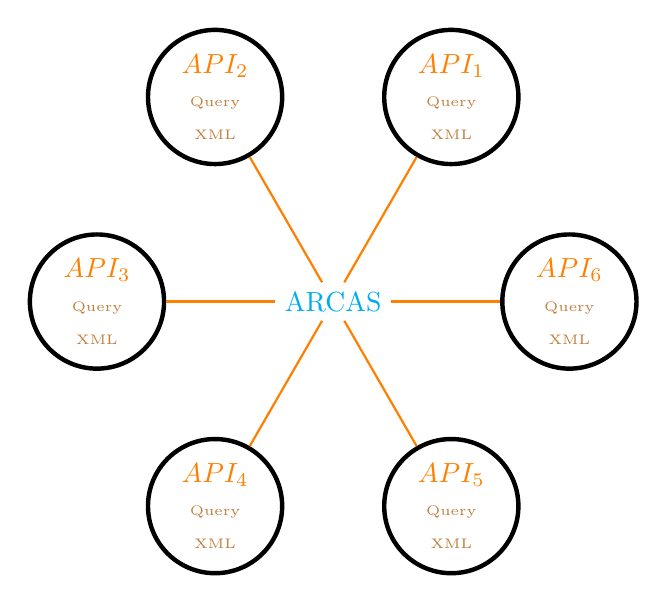
\begin{tikzpicture}

    \node[text=cyan] (center) at (0,0) {ARCAS};
\foreach \phi in {1,...,6}{
    \node[state, align=center, ultra thick] (v_\phi) at (360/6 * \phi:3cm) {\color{orange}$API_\phi$ \\ \color{brown}\tiny{Query}
    \\ \color{brown}\tiny{XML}};
         \draw[orange, thick] (v_\phi) -- (center);
}
\end{tikzpicture}
    \end{center}
\end{frame}

\begin{frame}[fragile]
    \begin{minted}
    [
    framesep=4mm,
    baselinestretch=1.2,
    bgcolor=DarkGray,
    fontsize=\small,
    ]
    {python}
import arcas

arguments = {'-a': None, '-t': 'Namibia',
             '-s': None, '-r': 1, '-y': None, '-b': None}

api =  arcas.Ieee()

parameters = api.parameters_fix(arguments)

url = api.create_url_search(parameters)
request = api.make_request(url)
response = api.get_root(request)
root = api.get_root(response)
raw_article = api.parse(root)
article = api.to_dataframe(raw_article)
    \end{minted}
\end{frame}

\begin{frame}[fragile]
    \begin{minted}
    [
    framesep=4mm,
    baselinestretch=1.2,
    bgcolor=DarkGray,
    fontsize=\tiny,
    ]
    {python}
import arcas

arguments = {'-a': None, '-t': 'Namibia', '-s': None,
             '-r': 100, '-y': None, '-b': None}

for p in [arcas.Ieee, arcas.Plos, arcas.Arxiv,
          arcas.Nature, arcas.Springer]:
    api = p()
    parameters = api.parameters_fix(arguments)

    url = api.create_url_search(parameters)
    request = api.make_request(url)
    response = api.get_root(request)
    root = api.get_root(response)
    raw_article = api.parse(root)

    for art in raw_article:
        article = api.to_dataframe(raw_article)
        api.export(articles, 'results.json')
    \end{minted}
\end{frame}

\begin{frame}[fragile]
    \begin{minted}
        [
        framesep=2mm,
        baselinestretch=1,
        bgcolor=DarkGray,
        fontsize=\tiny,
        ]
        {python}
{"key":{"0":"Momose2011",
        "1":"Momose2011",
        "2":"Momose2011"},
"unique_key":{"0":"4061b0ca3b823f85a0cb2823a554c524",
              "1":"4061b0ca3b823f85a0cb2823a554c524",
              "2":"4061b0ca3b823f85a0cb2823a554c524"},
"title":{"0":"Mapping pegmatite using HyMap data in southern Namibia",
         "1":"Mapping pegmatite using HyMap data in southern Namibia",
         "2":"Mapping pegmatite using HyMap data in southern Namibia"},
"author":{"0":"Atsushi Momose",
          "1":"Atsushi Momose",
          "2":"Atsushi Momose"},
"abstract":{"0":"A pegmatite deposit is an ..."},
"date":{"0":2011,
        "1":2011,
        "2":2011},
"journal":{"0":"2011 IEEE International Geoscience and Remote Sensing Symposium",
           "1":"2011 IEEE International Geoscience and Remote Sensing Symposium",
           "2":"2011 IEEE International Geoscience and Remote Sensing Symposium"},
"pages":{"0":"2216-2217",
         "1":"2216-2217",
         "2":"2216-2217"},
"key_word":{"0":"data analysis",
            "1":"geophysical image processing",
            "2":"geophysical techniques"},
"provenance":{"0":"IEEE",
              "1":"IEEE",
              "2":"IEEE"}}
     \end{minted}
\end{frame}

\begin{frame}
\begin{center}
\begin{figure}[H]
    \tikzstyle{arrow} = [thick,->]

\begin{center}
\begin{tikzpicture}[remember picture,
  inner/.style={draw=blue!70,thick,inner sep=3pt},
  outer/.style={draw=yellow!70,thick,inner sep=10pt}
  ]
  \node[outer,minimum width=15mm, minimum height = 4mm] (A) {
    \begin{tikzpicture}
      \node (ieee)  {IEEE};
      \node [right=of ieee] (nature) {Nature};
      \node [below=of ieee] (plos) {PLOS};
      \node [below=of nature] (plos) {...};
    \end{tikzpicture}
  };
  \node[outer, minimum width=15mm , minimum height = 1cm,left=2.7 cmof A,yshift=10mm] (B) {tools.py};
  \node[outer, minimum width=0.05*\columnwidth, minimum height = 2mm ,below=of B, inner sep=3pt, anchor=east] (C) {doc/};
  \node[draw=yellow!70, minimum width=0.05*\columnwidth, minimum height = 2mm, left=2 cmof A, inner sep=3pt, yshift=-30mm] (D) {arcas.readthedocs.io/};

  \node[outer,minimum width=15mm, minimum height = 7mm, below= of A] (F) {
    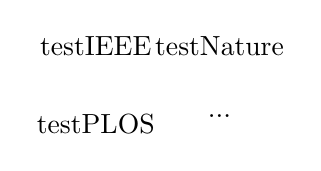
\begin{tikzpicture}
      \node  (ieee)  {testIEEE};
      \node [ right=of ieee, xshift=-1.2cm] (nature) {testNature};
      \node [ below=of ieee, yshift=0.5cm] (plos) {testPLOS};
      \node [ below=of nature, yshift=0.5cm] (plos) {...};
    \end{tikzpicture}
  };
  \draw [arrow] (C) -- ++(0,-30pt) -- ++(-55pt,0pt) |- (D);
\end{tikzpicture}
\end{center}
\end{figure}
\end{center}
\end{frame}

\begin{frame}[fragile]
    \begin{minted}
    [
    framesep=2mm,
    baselinestretch=1.2,
    bgcolor=DarkGray,
    fontsize=\tiny,
    ]
    {python}
arcas_scrape -h

Arcas. A library to facilitate scraping of APIs for scholarly resources.

Usage:
    arcas_scrape  [-h] [-p API] [-a AUTHOR] [-t TITLE] [-b ABSTRACT]
    [-y YEAR] [-r RECORDS] [-s START] [-v VALIDATE] [-f FILENAME]
    arcas_scrape --version


Options:
    -h --help              Show this
    --version              Show version.
    -p API                 The online API, from a given list, to parse [default: arxiv]
    -a AUTHOR              Terms to search for in Author
    -t TITLE               Terms to search for in Title
    -b ABSTRACT            Terms to search for in the Abstract
    -y YEAR                Terms to search for in Year
    -r RECORDS             Number of records to fetch
    -s START               Sequence number of first record to fetch
    -v VALIDATE            Checks if query returned with arguments asked [default: False]
    -f FILENAME            Name of json file [default: results.json]


    \end{minted}

\end{frame}

\begin{frame}
	\begin{center}
		\large\textbf{I academic API so you don't have to!}\\~\\
		\small{@NikoletaGlyn}\\
		\small{https://github.com/Nikoleta-v3/Arcas} \\
		\small{@SoftwateSaved} \\
		\small{@PhoenixCUni}
	\end{center}
\end{frame}

\end{document}




